\section{Plugins}

A plugin is a way of extending \espina{} functionality. It can
add a new element to the program, be it a new renderer, widget or
extension. \\
This section will document just the plugins included with \espina.

\subsection{Counting Region plugin}

A ``counting region'' is a volume for counting synapses. The boundaries of this
volume are marked red or green, indicating that a synapse touching the green boundary
will be marked as inside the volume and will be counted. On the other side a synapse
touching the red boundary wont be counted. Obviously the synapses inside of the volume
will be counted and the ones outside won't.\\
\espina{} will allow the existance of various regions for counting, each of one will
define it's own exclusion and inclusion boundaries.\\
This plugin will add representations to the corresponding planar views and will add a 
renderer to the three-dimanensional view. A widget will be added to the main widgets list 
so the user can create, modify and define the type of region.\\

\begin{figure}[H]
\centering
\includegraphics[scale=0.5]{fig/plugin-ct-2Dwidget.png}
\caption{Two-dimensional view showing one counting region boundaries for this view.}
\end{figure}

The two-dimensional representations will allow the user to modify the definition of the
boundaries by left-clicking and dragging them around, while the three-dimensional
representation will just show these boundaries.\\

\begin{figure}[H]
\centering
\includegraphics[scale=0.5]{fig/plugin-ct-widget.png}
\caption{Counting Region widget.}
\end{figure}

The counting region widget allow the user to manually edit the type and boundaries of several
counting regions.\\

\begin{tabular}{| m{1.3cm} | m{12cm} |}
\hline
\textbf{Button} & \textbf{Description}\\
\hline
Margins & Manually set left, right, top, bottom, upper and lower margins.\\
\hline
Type & Defines the type of the region.\\
\hline
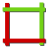
\includegraphics[width=0.7cm]{../../plugins/CountingRegion/rsc/apply} & Creates a new region of the selected type.\\
\hline
\includegraphics[width=0.7cm]{../../plugins/CountingRegion/rsc/trash-full} & Deletes the region selected in the region selection list.\\
\hline
Selection list & Selection box shows the margins and type of the region.\\
\hline
Region description & Lists the properties of the region.\\
\hline
\end{tabular}
\vspace{0.3cm} 

A counting region can be defined as:
\begin{itemize}
\item \textbf{Rectangular:} The region volume is largest possible parallelogram that encloses all the slices.
\item \textbf{Adaptative:} The region volume is the smallest possible, adapting it's boundaries to every slice.
\end{itemize}

